\documentclass[../thesis.tex]{subfiles}
\graphicspath{{\subfix{../Images/}}}

\begin{document}
\section{RQa: How do we best measure the energy consumption of a SNNI?}
% \begin{quote} \emph{RQa: How do we best measure the energy consumption of a SNNI?} \end{quote}

In this thesis, I found that Scaphandre is a good way to measure the energy consumption of a program or process in general, without the need of hardware. Therefore, Scaphandre is also an effective tool to measure the energy consumption of SNNI. Scaphandre has many possibilities and provides many options for the user. One could use Scaphandre to measure the energy and power usage of other processes, in the research on SNNI, but also in other fields. Unfortunately, remarkably few other options have been found to measure the power/energy consumption of a program or process. Besides, most solutions are language based, and not all languages do have options. For the c programming language, for example, no approaches have been found. It was therefore not possible to test the measurements of Scaphandre. It is important to lower the energy usage, for the environment and the fight against climate change, but also to oppose increasing energy prices and increase the usefulness of mobile devices. A future direction of work is therefore to create means to measure energy or power consumption, for both language specific programs and programs in general.

\section{RQb: How does the bandwidth influence the energy consumption of Cheetah and CrypTFlow2?}
% \begin{quote}
%     \emph{RQb: How does the bandwidth influence the energy consumption of a SNNI?}
% \end{quote}
In \autoref{section:rqb}, I described how I measured the energy consumption of both Cheetah, and CrypTFlow's HE class: $SCI_{HE}$. First, I measured the energy consumption of the SNNIs without any communication overhead. I will discuss the results in \autoref{subsection:discuss_power}. After getting the results of these measurements, I could measure how the bandwidth influences the energy consumption. I will discuss the results \autoref{subsection:discuss_bandwidth}.
\subsection{Power Consumption experiment}\label{subsection:discuss_power}
\begin{figure}[ht]
    \centering
    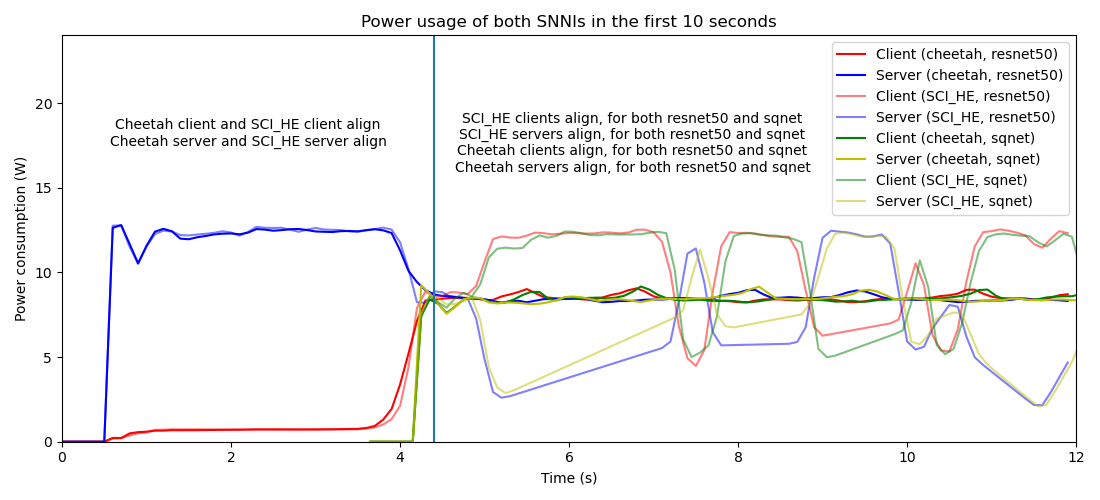
\includegraphics[width=.8\linewidth]{Thesis/Images/mean_first10secs.png} 
    \caption{First 12 seconds of both SNNIs and both NNs. Sqnet graph is shifted 3.6 seconds (duration of the Eigen phase).}
    \label{fig:first10secs}
\end{figure}
In the figures of the \textbf{Power Consumption experiment}, there seems to be an offline phase for both Cheetah and $SCI_{HE}$. The logs show that in the first 10 seconds, Cheetah is synchronising the silent OT pack, on which Cheetah heavily relies \parencite[p. 4]{cheetah}. This explains why the average consumption is low, since this phase does not rely on heavy computation, but rather on communication. Compared to for example Convolution layers, it makes sense that this phase uses less power. $SCI_{HE}$, on the other hand, uses kkot in approximately the first 20 seconds. Kkot needs more time, and relies more on computation than silent OT, which explains why the offline phase is longer compared to Cheetah.

An intriguing fact is that, although one can expect the logs of resnet50 and sqnet to differ in the first seconds (as a result the peak before the offline phase in the case of resnet50), the opposite is true. The logs of resnet50 and sqnet are the same in the first few seconds. Even the amount of data sent in the first few seconds is identical. A possible explanation could be that this peak in power usage before the offline phase is caused by the Eigen package \footnote{See README.md file in the Cheetah GitHub project}, used for matrix multiplication (matmul) layers. Both logs show that Cheetah and $SCI_{HE}$ are using the Eigen package for matmul, although sqnet does not have matmul layers according to the logs. Resnet50, on the other hand, does have matmul layers according to the logs. If the first 10 seconds of both NNs are graphed, and the graph of sqnet is shifted a few seconds (\autoref{fig:first10secs}), one can see that the Eigen package might explain the peak in power usage. Both the blue and light blue lines (server of both SNNI's on resnet50) and the red and light red lines (client of both SNNI's on resnet50) align almost perfectly. This demonstrates that the first approximately 4 seconds for both Cheetah and $SCI_{HE}$ in the case of resnet50 is also an offline phase. It is not certain if this is caused by the Eigen package, but this would be a plausible explanation since sqnet does not have matmul layers, while resnet50 has. Future work could measure the power consumption of other NNs, with and without mammul layers, to see if the Eigen package is indeed the cause. After approximately 4 seconds, the light colors (client and server of $SCI_{HE}$) and all the dark colors (client and server of Cheetah) align. This confirms another offline phase for the Silent OT pack and kkot. These offline phases could be improved to reduce the 'base' energy consumption of SNNI protocols. 

The constant consumption for Cheetah (with some peaks and troughs) can be explained, because Cheetah splits the big tensor and kernel into smaller blocks \parencite[p. 8]{cheetah}. Subsequently, Cheetah does perform mostly small calculations, which consume less power. Although CrypTFlow2 reduces the number of homomorphic rotations needed compared to prior work, it still utilizes expensive rotations, which causes the power consumption to be high. Alternately, it is still uncertain what layers cause the peaks and troughs after the offline phases, which makes it an interesting topic for further research. The logs do provide information on what layer the inference process is currently in, which can be displayed over the power consumption graph to determine the most power consuming layers.

In the figures, one could see that there is a difference between the power consumption of the client and the server. Again, it is uncertain what causes this difference, and what causes $SCI_{HE}$s server to consume almost double the power of $SCI_{HE}$s client. This difference will probably be explained when the layers are displayed over the power consumption graph. 

To conclude, I found that the server for Cheetah consumes less power and energy than the server for $SCI_{HE}$ with these measurements. Although the client consumes more power for Cheetah than $SCI_{HE}$, the energy consumption is lower. The total energy consumption is lower for Cheetah compared to $SCI_{HE}$. Additionally, I found that different phases can be identified in the figures, e.g. the communication phase. These different phases consume various amount of power. Future research can focus on what layers of the NN are being calculated by the protocol, and then connecting these measurements to the power readings. Layers that consume a great amount of power can then be identified and improved. Moreover, the ratio between power usage between the client and the server is shown in this thesis, but the cause can be investigated in future research. 

\subsection{Bandwidth experiments}\label{subsection:discuss_bandwidth}
These results show that bandwidth does have effect on the energy consumption of SNNI. It also shows that Cheetah is not only faster, but also more efficient in terms of energy compared to $SCI_{HE}$. Moreover, the improvement increases when limiting the available bandwidth for the client. Since this is a more realistic scenario than limiting the available bandwidth of the server (see \autoref{subsection:setup}), users of MLaaS would probably prefer Cheetah over $SCI_{HE}$.

As one can see in \autoref{fig:avg_energy}, the energy consumption increases considerably after a certain point. For Cheetah this point is with 100 Mbps available, while this point is at a limit of 50 Mbps for $SCI_{HE}$. Cheetah can handle lower generations compared to $SCI_{HE}$. Additionally, run-time increased before this turning-point, while energy consumption remained (almost) constant. The difference between the improvement when limiting the available bandwidth of the client with the improvement when limiting the available bandwidth (as can be seen in the \autoref{subsection:lowerbw}) can be explained. The server is responsible for 70\% of the total data sent for Cheetah, while for $SCI_{HE}$ this is only 50\%. This means that when the outgoing bandwidth of the server is limited, Cheetah will be relatively more impacted compared to $SCI_{HE}$. We can also see this in \autoref{fig:avg_energy}. The energy consumption of Cheetah increases more when the available bandwidth of the server limited, compared to when the client's bandwidth is limited. With $SCI_{HE}$, on the other hand, the increment of energy consumption is (almost) equal since the data sent is evenly distributed. This would also explain the increment in improvement for the server when limiting the client's bandwidth. Cheetahs client sends less data, both relatively compared to the server and in absolute terms compared to $SCI_{HE}$s client. When the outgoing bandwidth is limited, Cheetahs client will not be as much affected as $SCI_{HE}$s client. This is also why the improvement when limiting the server's outgoing bandwidth is not increasing since Cheetah's server is more affected. Since limiting the egress communication of the client is more realistic, and one can see a relation between energy improvement and bandwidth limits, programmers should keep in mind to keep the egress communication of the client in the SNNI process as low as possible. Besides, future work could investigate the turning point. By measuring the bandwidth used at certain time intervals, one could determine why the turning-points in the energy consumption is caused at certain bandwidth limits. 

I have tried to investigate why the bumps, caused after limiting the client's bandwidth, occur. Unfortunately, this cannot be explained by the time when the tests were performed since the experiments were performed at times when no other devices used the router. The run-times also do not have curious characteristics. I have not found the reason why this phenomenon occurs while limiting the client's bandwidth. Future work could investigate this phenomenon further.

This work shows the importance for the programmer to investigate the available bandwidth, and keep this in mind while creating better approaches of SNNI. This work can be used to create more energy efficient SNNI protocols. With my scripts, one only has to change the \verb|run-server.sh| and \verb|run-client.sh| with its own approach to measure the energy consumption of its own SNNI approach. This simplifies the research to energy efficient SNNI protocols. I hope that, since no prior works have been found in this area, my work will help programmers to make energy efficient protocols.

\section{Threats to internal validity}
Although I tried to limit traffic trough the router and tried to get it as close as 0, it is not certain that no other traffic might have passed trough. This could have influenced the bandwidth limit. I.e. when more traffic has passed the router, the available bandwidth would have been lower, and thus influenced the limit. More tests need to be done to validate the results, but unfortunately I do not have access to a router with no other traffic. But since the other traffic is close to zero, the results wont be influenced to a great extent.

One other remark to keep in mind is that when lowering the available bandwidth, run-time increases (see \autoref{fig:graph_times_mean}). Scaphandre writes the measurements to a file, but also saves data in higher hierarchical memory like RAM. Running Scaphandre for a long time will cause more reads and writes to lower and higher hierarchical memory. This results in reduced available memory for the SNNI protocol, which in turn will cause the protocol to read and write more to this memory. This might have impact on the energy consumption since run-time increases. Scaphandre does not measure the energy consumed for reading and writing data, so this would be an interesting topic for future research. 

\section{threats to external validity}
Since the measurements of the \textbf{Power Consumption experiments} are done 50 times, with little to no influence from the 'outside' (i.e. no communication overhead), findings are reliable. And although tests are only done with two NNs, and the results can therefore not be generalised, the experimental results show interesting topics for future research. The results of the \textbf{Bandwidth experiments} are only done a small amount of times and with only one NN, and can therefore not be generalised. This framework provides the support for 2 other NNs: ResNet50 and DenseNet121. Unfortunately, I did not have enough time to test other NNs. Future work could extend this research by measuring the implications of bandwidth on the energy consumption of these two NNs. Besides, as said earlier, scripts can be easily adapted to other approaches of SNNI to generalise results. 

Additionally, experiments are only performed in the LAN environment. More realistic scenarios of MLaaS often have more links and devices between client and server. These links and devices could also be a bottleneck in the whole communication process. Besides, extra links would increase the ping time between server and client. This has influence on the run-time and could therefore have implications on the energy usage. Besides, experiments are done in optimal conditions, e.g. client that is close to the router, high-end router, no walls between the wireless connection of router and client, cable connection between router and server, etc. 

% \color{red} revisit the research questions\color{black}
\section{Ethics}
No ethics are involved in this thesis, other than the moral duty to reduce energy consumption. If one does not have this duty, one might question the importance of this research. 
\end{document}